\documentclass[../sparc.tex]{subfiles}
\graphicspath{{\subfix{../images/}}}
\begin{document}

%%%%%%%%%%%%%%%%%%%%%%%%%%%%%%%%%%%%%%%%%%%%%%%%%%%%%%%%%%%%%%%%%%%%%%%%%%%%%%%%
\newpage
\section{Bass clef}
\index{Music!Bass clef}

Aside from the treble clef, there's also the \emph{bass clef}.  Usually bass
clef is used for those musical instruments that have lower frequency range that
are covered by the treble clef.

\begin{figure}[ht]
  \centering
  \begin{tikzpicture}
    \node (image) at (2, 0) { \resizebox{1.0\textwidth}{!}{
        \begin{lilypond}
          \relative c {
            \clef "bass"
            \numericTimeSignature
            \time 4/4
            c8 d8 e8 f8 g8 a8 b4
          }
        \end{lilypond}
      }
    };
    \foreach \n [count=\i, evaluate=\i as \y using real(\i / 2.55)] in {
      E2, G2, B2, D3, F3, A3
    } {
      \node at (-3.3, \y - 1.5) {\tiny \n};
    };
    \foreach \n [count=\i, evaluate=\i as \y using real(\i / 2.55)] in {
      F2, A2, C3, E3, G3, B3
    } {
      \node at (-3.0, \y - 1.3) {\tiny \n};
    };
    \draw[thick, ->] (-4.0, -2.0) -- (8.0, -2.0) node[anchor=north east] {x};
    \draw[thick, ->] (-4.0, -2.0) -- (-4.0, 1.5) node[anchor=north east] {y};
  \end{tikzpicture}
  \caption{A musical ``graph'' for the bass clef.  The ``x'' axis represents the
    time, and the ``y'' represents the sound frequency.}
  \label{fig:lilypond-bass-clef}
\end{figure}

On the fig. \ref{fig:lilypond-bass-clef} the layout of the notes in the bass
clef is shown.

\begin{figure}[ht]
  \centering
  \begin{tikzpicture}
    \node (image) at (4, 2) {
      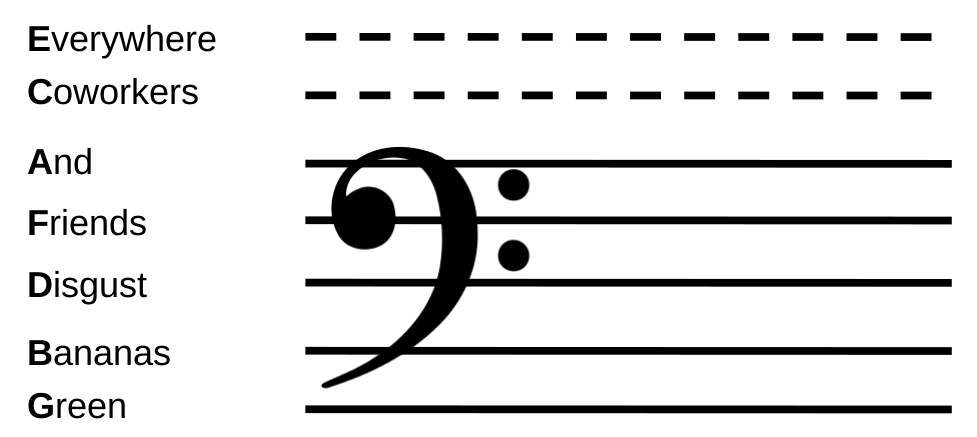
\includegraphics[width=8cm]{music-bass-clef-mnemonic}
    };
    \draw[thick, ->] (0, -1.0) -- (10, -1.0) node[anchor=north east] {x (Time)};
    \draw[thick, ->] (0, -1.0) -- (0, 4.0) node[anchor=north east] {y (Frequency)};
  \end{tikzpicture}
  \caption{A mnemonic to remember the position of notes in the bass clef.}
  \label{fig:lilypond-bass-clef-mnemonic}
\end{figure}

A mnemonics for remembering the position of notes in the bass clef is shown in
fig. \ref{fig:lilypond-bass-clef-mnemonic}.

\end{document}
